\documentclass[10pt]{article}

\usepackage[margin=1.05in]{geometry}
\usepackage{lmodern}
\usepackage[T1]{fontenc}
\usepackage{microtype}
\usepackage{graphicx}
\usepackage{booktabs}
\usepackage{amsmath}
\usepackage{amssymb}
\usepackage{xcolor}
\usepackage{caption}
\usepackage{float}
\usepackage[colorlinks=true, linkcolor=black, citecolor=black, urlcolor=blue!50!black]{hyperref}

\hypersetup{
  pdftitle={Fast-Weight Memory Layers Improve Small Language Models at Matched Parameters and Compute},
  pdfauthor={Dimitar Stojanovski},
  pdfsubject={Machine Learning},
  pdfkeywords={fast-weight memory, delta rule, linear attention, gated DeltaNet, chain-of-thought, small language models, matched-compute evaluation}
}

\captionsetup{font=small, labelfont=bf, skip=6pt}
\setlength{\parskip}{2pt}

\title{\vspace{-1.2em}\Large\bf Fast-Weight Memory Layers Improve Small Language Models\\at Matched Parameters and Compute\vspace{-0.3em}}
\author{\normalsize Dimitar Stojanovski\\[-1pt]\small Aware AI Labs \quad \texttt{dimitar@awareailabs.com}}
\date{\small July 2026}

\begin{document}
\maketitle
\vspace{-1.6em}

\begin{abstract}
\noindent
We replace every second attention layer of a modern Transformer with a gated
delta-rule fast-weight memory layer and evaluate the result under strict
accounting: parameters matched to $0.1\%$, identical data, matched training
budget, and pre-registered decision margins. On five procedural task families,
the memory hybrid is more accurate on all five ($+4.0$ to $+21.8$ points) while
spending $20$--$40\%$ \emph{fewer} inference FLOPs per correct answer
(Figure~\ref{fig:hero}). A $2{\times}2$ ablation attributes both effects to the
delta mechanism ($+22.8$) rather than its sliding-window component ($+3.5$);
doubling the baseline's training budget does not close the gap ($+25.8$ on
non-saturated difficulty tiers); and the preferred memory density is every
second layer. At 50M parameters under a fixed recipe the advantage is
task-dependent: it grows on program execution ($+31.7$) and reverses on state
tracking ($-5.2$). Pricing the mechanism against visible chain-of-thought at
matched per-answer FLOPs, trained rationale tokens win on accuracy --- a
FLOP-matched $1.7{\times}$ wider model buys nothing and contentless filler
tokens hurt --- yet the two mechanisms \emph{compose}: the hybrid with traces
reaches $100\%$ at ${\sim}5\%$ lower cost than the Transformer with traces.
We also characterize a bimodal training outcome: on a rule-revision task,
seeds transition discontinuously to ${\sim}100\%$ accuracy ($3/16$ fresh
seeds, plus $2$ caught mid-transition; $0/6$ for the baseline), with an
onset that is trajectory-nondeterministic; no early-training signal met the
pre-registered predictor bar. The complete study --- ten pre-registered
experiments including three negative results --- cost \$59 of commodity cloud
compute. Code, per-run results, and pre-registrations are
public.\footnote{\url{https://github.com/dimitri-sky/fast-weight-memory-lm}
(paper) and \url{https://github.com/dimitri-sky/aware-latent-depth} (full
research program, run-level ledger).}
\end{abstract}

\begin{figure}[H]
\centering
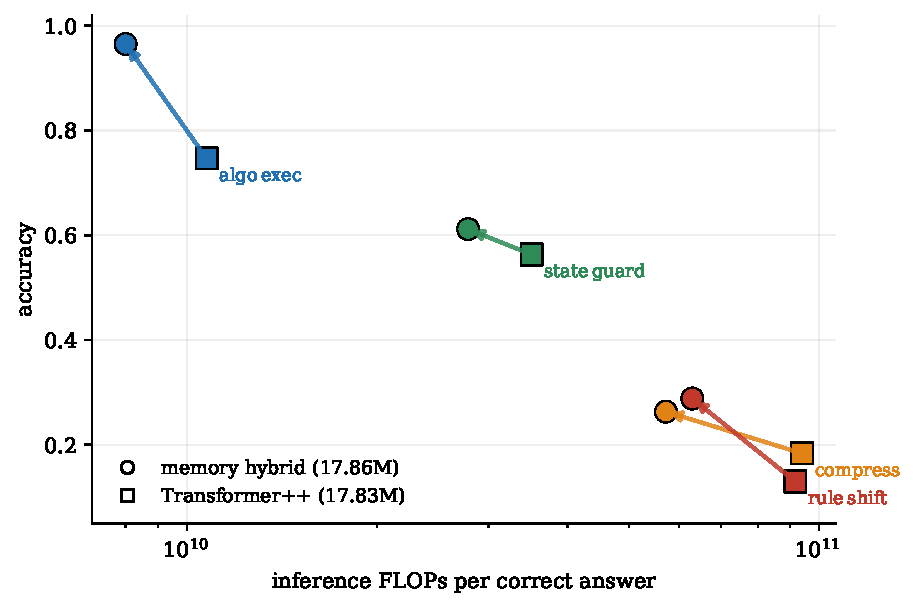
\includegraphics[width=0.68\linewidth]{figs/hero_pareto.pdf}
\caption{\textbf{Main result.} Accuracy versus inference FLOPs per correct
answer at 17.8M parameters, same data, same training budget (means over 3--6
seeds; arrows point from Transformer++ to the memory hybrid). The hybrid is
up-left --- more accurate \emph{and} cheaper per correct answer --- on every
family. (\texttt{dsl\_learn}, $+4.0$, omitted for legibility.)}
\label{fig:hero}
\end{figure}
\vspace{-0.6em}

\section{Introduction}

Linear-attention hybrids with delta-rule fast weights are entering production
language models, yet public evidence for \emph{why} they win is thin: papers
rarely hold parameters, data, and compute fixed simultaneously, and per-answer
inference cost is almost never reported. We contribute a small, fully audited
data point. The question is narrow and the accounting is strict; every claim
below was given a pre-registered pass/fail margin before results existed, and
every number traces to a run identifier in a public ledger. Beyond the
head-to-head, we price the mechanism against the two obvious alternatives at
matched per-answer FLOPs --- visible chain-of-thought tokens and a wider model
--- and against a weight-tied recurrent-depth architecture, so the reader gets
one consistent exchange rate between four ways of spending inference compute.

Concretely, we compare a byte-level Transformer++ baseline (RoPE, SwiGLU,
RMSNorm, GQA; 17.83M) against a hybrid that replaces every second attention
layer with a \emph{gated delta-rule fast-weight
layer}~\cite{fwp,gateddeltanet} --- a linear-attention state
$S_t \in \mathbb{R}^{d_k\times d_v}$ updated token-by-token with a
learned write/erase gate --- keeping sliding-window attention ($w{=}128$) on
the remaining layers (17.86M, $+0.1\%$; Figure~\ref{fig:arch}), the layer
pattern production hybrids have converged on~\cite{kimi}. Both are
trained from scratch, per-family, on SAGE: five generated,
contamination-audited procedural families (program execution, mid-session rule
revision, in-session codebook learning, state tracking, fresh-language
induction) with difficulty tiers and execution-checked scoring.

\begin{figure}[H]
\centering
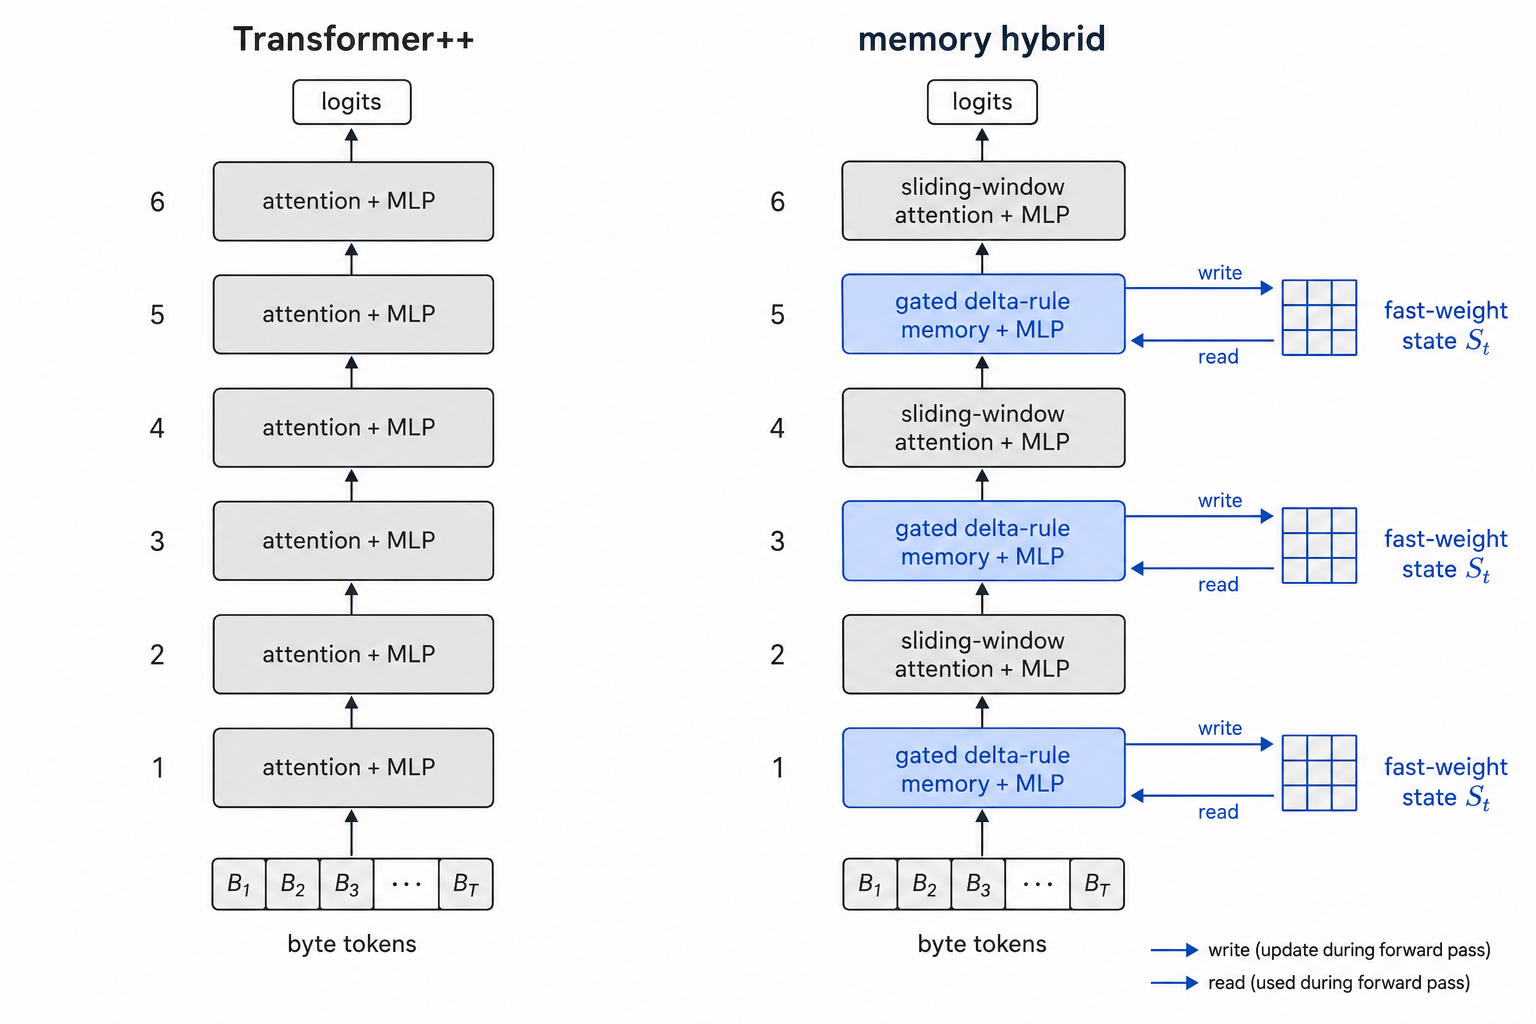
\includegraphics[width=0.9\linewidth]{figs/architecture_comparison.png}
\caption{The two architectures. Left: the Transformer++ baseline. Right: the
memory hybrid --- every second block is a gated delta-rule memory layer that
writes to and reads from a fast-weight state $S_t$ during the forward pass;
the remaining blocks use sliding-window attention ($w{=}128$).}
\label{fig:arch}
\end{figure}

\section{Setup}

\textbf{Accounting.} FLOPs are counted analytically (2 FLOPs per MAC) and
cross-checked against PyTorch's counter in CI (agreement within $10\%$
enforced). Every generated token is charged a full forward pass at its context
length. The efficiency metric is \emph{inference FLOPs per correct answer},
which charges mistakes to the model that makes them.

\textbf{Protocol.} 4{,}000 steps $\times$ batch 32 $\times$ 768 tokens
per family; learning rate depth-scaled; 3 seeds by default (2--16 where noted,
all stated in advance). Margins, gates, and deviations are logged in
time-stamped pre-registration files; every mid-study deviation (an arm dropped
for cost before its results existed; a config bug caught by a feasibility
probe; one session's results stranded by an infrastructure failure and re-run
before per-tier outcomes were seen) is recorded there at decision time.

\section{Results}

\subsection{The memory hybrid wins on all five families, at lower cost}

\begin{table}[h]
\centering\small
\caption{18M head-to-head. Mean accuracy $\pm$ SD over seeds; Welch $t$
reported per family. FLOPs/correct is inference cost per correct answer.
Superscripts give seed counts where they differ from 3.}
\label{tab:main}
\begin{tabular}{lccccc}
\toprule
family & Transformer++ & memory hybrid & $\Delta$ & Welch $t$ & FLOPs/correct ratio \\
\midrule
algo\_exec   & $.747\pm.016$ & $\mathbf{.965\pm.009}$ & $+21.8$ & $20.7$ & $0.75\times$ \\
rule\_shift$^{6\mathrm{s}}$ & $.130\pm.034$ & $\mathbf{.288\pm.349}$ & $+15.8$ & $1.1$ & $0.69\times$ \\
compress     & $.184\pm.009$ & $\mathbf{.263\pm.032}$ & $+7.9$  & $4.1$  & $0.61\times$ \\
state\_guard & $.563\pm.043$ & $\mathbf{.612\pm.028}$ & $+4.8$  & $1.7$  & $0.79\times$ \\
dsl\_learn$^{2\mathrm{s}}$   & $.165\pm.014$ & $\mathbf{.205\pm.021}$ & $+4.0$  & $2.2$  & --- \\
\bottomrule
\end{tabular}
\end{table}

\begin{figure}[h]
\centering
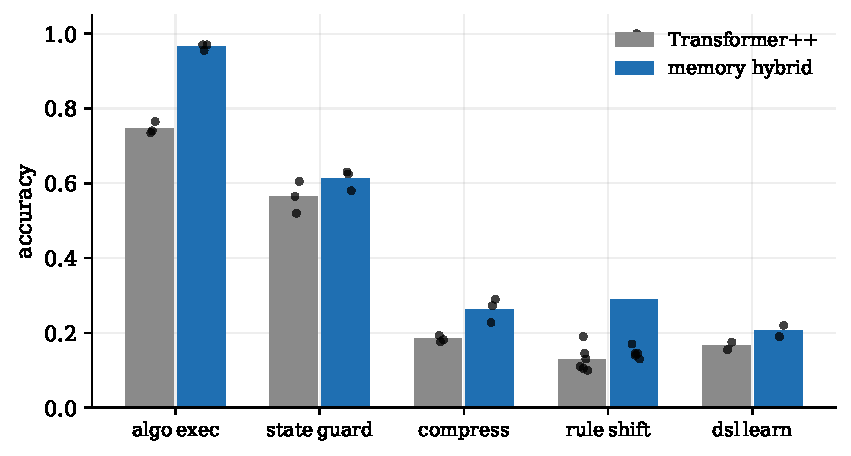
\includegraphics[width=0.8\linewidth]{figs/families.pdf}
\caption{Per-family accuracy with individual seeds (dots). The hybrid leads on
5/5 families; \texttt{rule\_shift}'s variance is the bimodality of
Figure~\ref{fig:grok}.}
\label{fig:families}
\end{figure}

The pooled family-mean gap is $+13.5$ points against a pre-registered
$+3.0$ margin. Statistical honesty: the gap is individually significant on the
two largest effects (algo\_exec $t{=}20.7$, compress $t{=}4.1$) and directional
but not individually significant on the rest at these seed counts;
\texttt{rule\_shift}'s mean is dominated by one grokked seed (median gap
$+2.5$). The pre-registered $2{\times}$pooled-SD stability gate fails for
exactly this reason, and we report it as such.

\subsection{Attribution: the delta mechanism, not the window}

The hybrid differs from the baseline in two ways, so we complete the
$2{\times}2$ (Figure~\ref{fig:attr}). Adding the sliding window alone moves the
baseline $+3.5$; adding delta layers alone moves it $+22.8$ ($.975$, slightly
\emph{above} the full hybrid); the interaction is $-4.5$. The window also fails
to reproduce any memory-family gain (state tracking \emph{degrades} by $4.1$).
A pre-registered prediction was falsified here: we expected the window to
explain the FLOP discount, but the discount is also delta-driven --- the window
trims only ${\sim}7\%$ of FLOPs; the rest comes through the accuracy
denominator.

\begin{figure}[h]
\centering
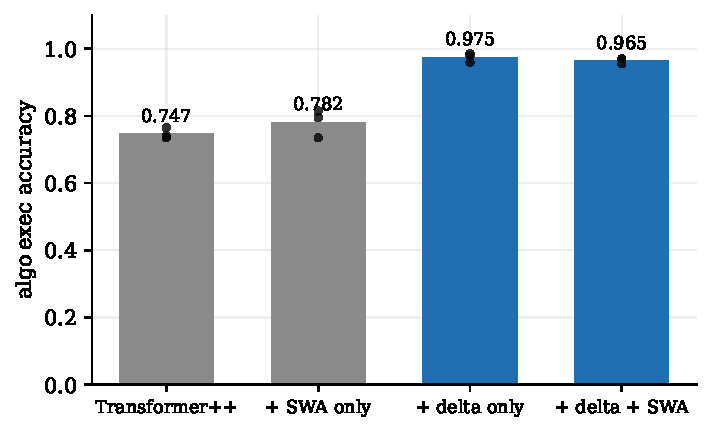
\includegraphics[width=0.62\linewidth]{figs/attribution.pdf}
\caption{$2{\times}2$ ablation on \texttt{algo\_exec} (3 seeds each, dots).
The delta mechanism carries the effect.}
\label{fig:attr}
\end{figure}

\subsection{Doubling the baseline's training budget does not close the gap}

If delta layers merely \emph{optimize faster}, more training should let the
baseline catch up. At $2\times$ steps the baseline improves ($.747\!\to\!.795$
--- the arm discriminates) but the gap on non-saturated tiers (3--5) remains
$+25.8$ points against a pre-registered pass bar of half the original gap
(Figure~\ref{fig:budget}). A ceiling guard (hybrid $>.95$ overall) moved the
primary read to hard tiers, as pre-registered.

\begin{figure}[h]
\centering
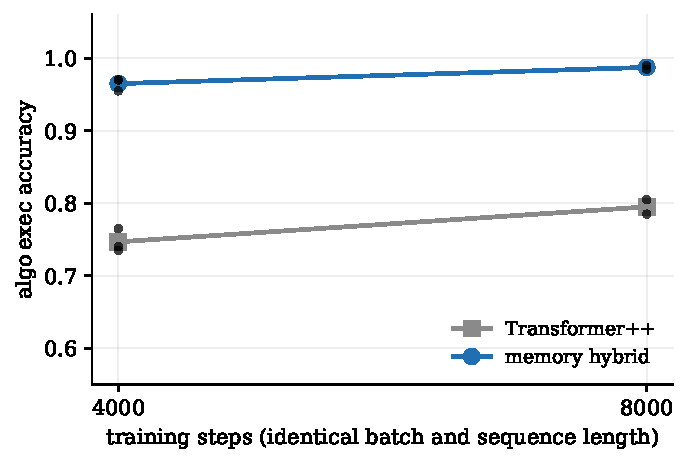
\includegraphics[width=0.56\linewidth]{figs/budget.pdf}
\caption{Training-budget robustness on \texttt{algo\_exec}.}
\label{fig:budget}
\end{figure}

\subsection{At 50M the advantage is task-dependent}

Scaling both models to 50.5M ($-0.05\%$ param match) under the same recipe:
the program-execution gap \emph{grows} to $+31.7$ while the state-tracking gap
\emph{reverses} to $-5.2$ (Figure~\ref{fig:scale}). A caveat cuts both ways:
the 50M baseline underperforms its own 18M counterpart on
\texttt{algo\_exec}, indicating the fixed recipe undertrains at this size ---
part of the growth is baseline weakness, and the reversal may be a tuning
artifact. We therefore make no uniform-scaling claim.

\begin{figure}[h]
\centering
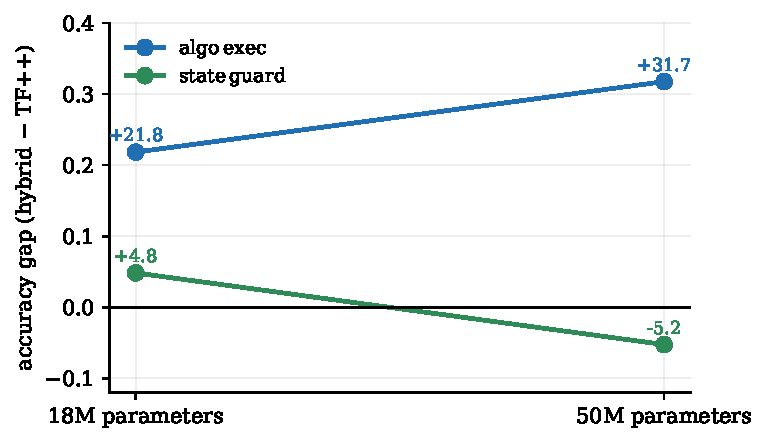
\includegraphics[width=0.56\linewidth]{figs/scale.pdf}
\caption{Accuracy gap at 18M vs.\ 50M (fixed training recipe, 2 seeds at 50M).}
\label{fig:scale}
\end{figure}

\subsection{Pricing latent memory against visible chain-of-thought}

Fast-weight memory is one way to buy computation at inference time; generating
rationale tokens is another, and whether latent computation can substitute for
visible traces is an open thread~\cite{coconut}. We price both on the same axis
(Figure~\ref{fig:cot}): Transformer++ variants trained to emit a
\texttt{THINK:}\,\ldots\,\texttt{ANSWER:} trace at three granularities
(the budget knob is trace granularity at training time --- eval-time
truncation is an invalid instrument, since a truncated trace never reaches
\texttt{ANSWER:}), a contentless length-matched filler control, and a
$1.7{\times}$ wider model ($30.76$M, $d{=}672$) sized analytically so its
direct per-answer FLOPs match the long-trace arm within $1.8\%$. Every
generated token is charged a full forward pass at its context length; the
primary read is tier 3--5 accuracy, all margins pre-registered at $+3.0$
points.

\begin{figure}[h]
\centering
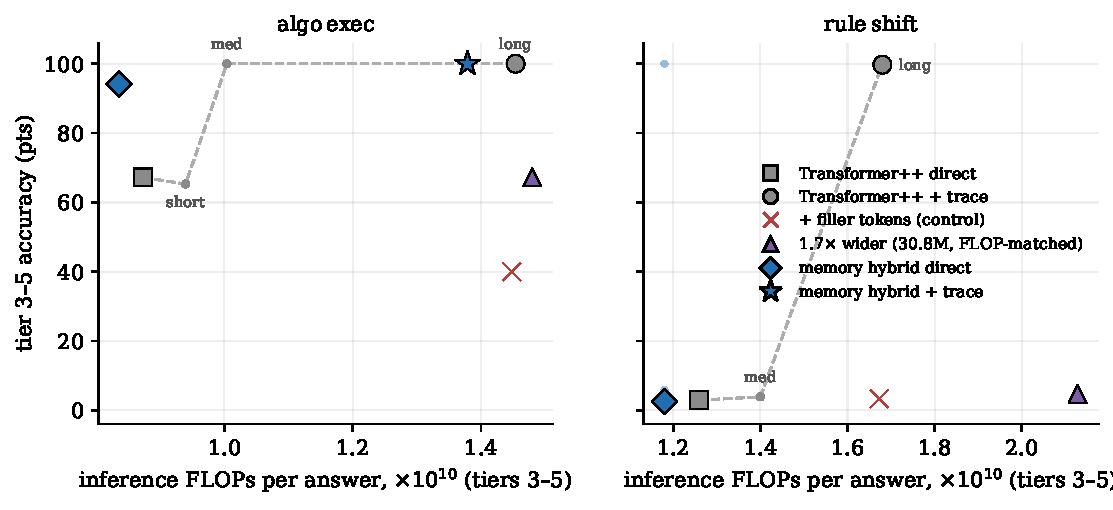
\includegraphics[width=0.98\linewidth]{figs/cot_exchange.pdf}
\caption{\textbf{Four ways to spend inference compute}, priced on one axis
(tier 3--5 accuracy vs.\ measured FLOPs per answer; trace granularity
annotated along the dashed budget curve). Small dots on
\texttt{rule\_shift}'s hybrid-direct marker are individual seeds --- the
median is plotted because of the bimodality of Figure~\ref{fig:grok}.}
\label{fig:cot}
\end{figure}

Four pre-registered gates, all decisive. \textbf{(1) Trained traces pay:}
$+32.8$ over direct on program execution (best budget) and $+96.8$ on rule
revision. \textbf{(2) The win is content, not compute:} filler tokens at
identical length and FLOPs are null on rule revision ($+0.4$) and
\emph{negative} on program execution ($-27.2$) --- no pause-token~\cite{pause}
free lunch at this scale. \textbf{(3) Tokens beat parameters:} the FLOP-matched wider
model buys $+0.0$ and $+1.8$ over its own 17.8M baseline. \textbf{(4) Visible
beats latent on accuracy, and the crossover is cheap:} the hybrid holds a
27-point edge over the direct baseline at $0.96\times$ its cost, but a
medium-granularity trace passes it ($100.0$) at $1.20\times$ the hybrid's
FLOPs; on rule revision the full-table trace converts the grokking lottery of
\S\ref{sec:grok} into $99.7$ on every seed --- traces buy \emph{reliability},
not just accuracy. Accuracy is not monotone in trace budget: sparse
every-third-step traces score at or below direct ($65.3$), so the trace's
step-by-step structure, not its token count, carries the effect.

The mechanisms compose rather than compete: the memory hybrid trained with
long traces reaches $100.0$ on all tiers, both seeds, at ${\sim}5\%$ fewer
FLOPs per answer than the Transformer++ with the same traces --- the trace
does the heavy lifting and the delta layers trim the cost. Scope: trained,
task-aligned, in-distribution rationales under greedy decoding; the FLOP axis
spans only $1.0$--$1.7\times$ direct because prefill dominates at these
prompt shapes --- itself a deployment-relevant observation (short-prompt
regimes price visible reasoning very low).

\subsection{Bimodal skill acquisition, replicated}
\label{sec:grok}

On \texttt{rule\_shift}, five of six hybrid seeds land at $.13$--$.17$ and one
reaches $1.00$ (train loss $0.0014$) --- a discontinuous transition absent in
all six baseline seeds (Figure~\ref{fig:grok}). Same data, same
configuration, different initialization. Artifact checks: all twelve runs
share one eval split and scorer (a bug would inflate every seed); training
data is identical across seeds; the contamination audit passed; and the
transition is visible in the training loss, not only the eval score.

A pre-registered replication on 16 fresh seeds (disjoint seed range,
byte-identical config) confirms the phenomenon: $3/16$ grok (Wilson 95\% CI
$[.07,.43]$, consistent with the original $1/6$), two more are caught
mid-transition when the 4{,}000-step budget ends ($.885$, $.64$), and eleven
stay flat. Instrumented probes place transition onsets at steps
1{,}000--2{,}600, so ``rare discrete event'' is better read as ``slow
transition that often does not fit the budget.'' A same-seed re-run of the
original grokked seed reached only $.695$ --- onset is
trajectory-nondeterministic, not seed-determined. The predictor question came
back negative: across seven pre-registered early-training signals (loss
curvature, gradient norms, fast-weight state norm and effective rank, gate
drift, weight-norm ratios, early tier-1 probe accuracy), none separated
grokked from flat runs at the pre-registered bar within the first 1{,}000
steps --- a $k{=}2$ state-norm separation broke at $k{=}3$.

\begin{figure}[h]
\centering
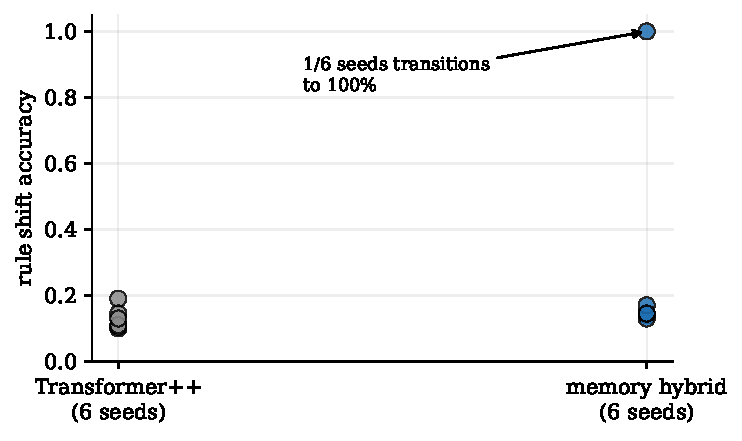
\includegraphics[width=0.72\linewidth]{figs/grok.pdf}
\caption{Seed-level outcomes on \texttt{rule\_shift}: the original 6-seed
head-to-head and the pre-registered 16-seed replication (fresh seeds,
identical config).}
\label{fig:grok}
\end{figure}

\subsection{Negative control: recurrent depth does not pay here}

For completeness: in the same program, weight-tied loop
architectures~\cite{huginn,ouro} (prelude--core$\times K$--coda) failed to pay
their FLOP cost twice --- vanilla loops lose to a step-matched control
(consistent with independent iso-FLOP analyses~\cite{sparselayers}), and the
current best training recipe (per-loop supervision~\cite{lotus}, randomized
loop counts, truncated BPTT~\cite{rdvla}) twice produced \emph{loop-invariant}
models, detected only by a pre-registered diagnostic that evaluates the same
checkpoint at $K{=}1$ vs.\ $K{=}4$ ($<2$-point gap against a 5-point gate) ---
the readout blind spot of~\cite{blindspot}. Latent computation helped here
only when it carried \emph{writable state across the sequence}, not when it
re-applied the same transformation in depth.

\section{Limitations}

15--50M scale; procedural byte-level benchmark; per-family specialists (no
multi-task control); one window size; 2--16 seeds per arm; the 50M recipe
untuned. The chain-of-thought comparison measures trained, in-distribution
rationales under greedy decoding --- not prompted or noisy ones --- and its
training FLOPs are reported but not matched across arms (the claim is scoped
to inference-time economics, as pre-registered). The delta scan is implemented
sequentially, so wall-clock favors the baseline (FLOP counts are
implementation-independent; chunked-parallel kernels for this layer family
exist in production systems). Small-scale results do not license frontier
claims; the mechanism family is already validated at scale by others --- what
this study adds is the controlled, matched, pre-registered evidence chain and
the per-answer cost accounting.

\section{Reproducibility}

All pre-registrations (\texttt{agent/log/EXP-*.md}), the 1{,}600-row run
ledger (\texttt{experiments/results.csv}), frozen configs, adjudication
scripts, and a two-minute demo (\texttt{scripts/demo.py}: fresh puzzles, both
models side-by-side, live FLOPs-per-correct meter) are public. Total compute:
one local RTX~3080 plus commodity RTX~5090 pod-hours; \${}59 across the two
study arcs (\${}38 architecture, \${}21 chain-of-thought economics and
grokking replication).

\vspace{2pt}
\noindent{\small This work is licensed under a Creative Commons Attribution
4.0 International License (CC~BY~4.0).}

\begin{thebibliography}{11}\small
\bibitem{gateddeltanet} S.~Yang et al. Gated Delta Networks: Improving Mamba2 with Delta Rule. \emph{ICLR}, 2025. arXiv:2412.06464.
\bibitem{fwp} I.~Schlag, K.~Irie, J.~Schmidhuber. Linear Transformers are Secretly Fast Weight Programmers. \emph{ICML}, 2021. arXiv:2102.11174.
\bibitem{kimi} Kimi Team. Kimi Linear: An Expressive, Efficient Attention Architecture. 2025. arXiv:2510.26692.
\bibitem{pause} S.~Goyal et al. Think before you speak: Training Language Models with Pause Tokens. \emph{ICLR}, 2024. arXiv:2310.02226.
\bibitem{coconut} S.~Hao et al. Training Large Language Models to Reason in a Continuous Latent Space. 2024. arXiv:2412.06769.
\bibitem{huginn} J.~Geiping et al. Scaling up Test-Time Compute with Latent Reasoning: A Recurrent Depth Approach. 2025. arXiv:2502.05171.
\bibitem{ouro} Ouro team. Scaling Latent Reasoning via Looped Language Models. 2025. arXiv:2510.25741.
\bibitem{blindspot} Readout blind spot in per-loop supervised looped models. 2026. arXiv:2606.24898.
\bibitem{lotus} LOTUS: Latent Optimization via Step-Aligned Supervision. 2026. arXiv:2606.31779.
\bibitem{rdvla} Recurrent-Depth VLA: Implicit Test-Time Compute Scaling via Latent Iterative Reasoning. 2026. arXiv:2602.07845.
\bibitem{sparselayers} Sparse-Layers: iso-FLOP analysis of weight-tied depth, 16M--305M. 2026. arXiv:2605.09165.
\end{thebibliography}

\end{document}
